% ------------------------------------------------------------------------
% TCC_CC:   Modelo de Trabalho Monográfico Acadêmico UERN 
%           para o curso de Bacharelado em Ciência da Computação
%
% Esse template é baseado no template 
% desenvolvido por Francisco Reinaldo
% Disponivel em: https://pt.overleaf.com/latex/templates/utfpr-modelo-tcc-monografia-dissertacao-tese-com-pdf-a-3b-versao-goldendragon/znzmpctjxmqq)
%
% Sendo modificado para se encaixar 
% nos requisitos solicitados pela UERN no ano de 2020
%
% Caso você tenha caído de cabeça e não 
% entenda nada de overleaf, peça ajuda a
% quem indicou :P
%
% Ou der seus pulos e aprenda sozinho.
% Dá um google ai.
%
% Mais para dar um colher de chá eu coloquei alguns tutoriais :)
%
% A maioria dos dados (fora os texto em si)
% que você precisar modificar em relação ao o seu nome,
% orientador, data, banca estão no arquivo 
% dados-gerais dá uma olhada lá. Mas fique a 
% vontade para editar como quiser :).
%
% Desenvolvido por: Althierfson Tullio O aluno
%
% Versao de Controle: v32 - Codinome Externo: GoldenDragon
%
% ------------------------------------------------------------------------


% --- LianTze / Reinaldo´s Fine Tuning
\RequirePackage{scrlfile}
\AfterClass{memoir}{\usepackage[a-3b]{pdfx}} %v.3
%Para funcionar, deixe na raiz: sRGB_IEC61966-2-1_black_scaled
%\BeforePackage{hyperref}{\usepackage[a-3b]{pdfx}} %v.3.2
% ---

\documentclass[
	% -- opções da classe memoir --
	12pt,				% tamanho da fonte
	oneside,			% para impressão em frente. Oposto a twoside (frente,costas)
	a4paper,			% tamanho do papel. 
	%sumario=tradicional,
	% % -- opções da classe abntex2 --
	chapter=TITLE, % títulos de capítulos convertidos em letras maiúsculas
	%section=title,
	% -- opções do pacote babel --
	english,			% idioma adicional para hifenização
	brazil				% o último idioma é o principal do documento
	]{abntex2}

% --- 
% PACOTES PARA AJUSTE e CORREÇÕES EM ABNTEX2
% --- 
% ---
% Não tente entender este .tex
% Aqui tem ajustes hardcore sombreando ABNTEX2 para finos ajustes de ABNT.
% ---

% ---
% PDF/A
% ---
%
% PDF/A é um padrão ISO destinado ao arquivamento a longo prazo de documentos eletrônicos. Enfatiza a autonomia e a reprodutibilidade, bem como os metadados legíveis por máquina.
%
% A pedido da UTFPR-FB-Biblioteca, valide seu PDF/A em
% https://www.pdf-online.com/osa/validate.aspx
%
% PDF gerado estará ok se a mensagem for: "The document does conform to the PDF/A-3b standard."


% ---
% Pacotes básicos 
% ---

\usepackage[T1]{fontenc}		% Selecao de codigos de fonte.
\usepackage[utf8]{inputenc}		% Codificacao do documento -conversão automática dos acentos
\usepackage{ae,aecompl}
%http://dsanta.users.ch/resources/type1.html

\usepackage{helvet}			% Usa a fonte time new romam		
%\usepackage{lastpage}			% Usado pela Ficha catalográfica
\usepackage{indentfirst}		% Indenta o primeiro parágrafo de cada seção.
\usepackage{color}				% Controle das cores
\usepackage{subcaption, graphicx}			% Inclusão de gráficos
\usepackage{microtype} 			% para melhorias de justificação
\usepackage{titlesec}
\usepackage{lipsum}
\usepackage{fancyhdr}           % Para manipular o cabeçalhos
\usepackage{pdfpages}           % Para adicionar PDFs

% % ---
\hbadness=99999 %That's just TeX alerting you that it was unable to typeset your document perfectly. The \hbadness variable doesn't affect the typography at all; it just tells TeX the threshold for printing its annoying "Underfull \hbox (badness xxxx) in paragraph..." warnings. 

% ---
% Pacotes de citações
% ---
% \usepackage[brazilian,hyperpageref]{backref}	 % Paginas com as citações na bibl
\usepackage[brazilian]{backref}

%Sugestão
\usepackage[alf,bibjustif, 	
			abnt-emphasize=bf,
			bibjustif,
			recuo=0cm,
			abnt-url-package=url,
			abnt-refinfo=yes,
			abnt-repeated-title-omit=yes,
			abnt-full-initials=yes, %(yes) nome por extenso, (no) apenas iniciais
			abnt-etal-list=3,
			abnt-etal-cite=3,  %abreviar com mais de 3 autores
			abnt-nbr10520=2002,
			abnt-thesis-year=final
]{abntex2cite}



% --- 
% Espaçamentos entre linhas e parágrafos 
% --- 
%
% O tamanho do parágrafo é dado por:
\setlength{\parindent}{1.3cm}
%
% Controle do espaçamento entre um parágrafo e outro:
%\setlength{\parskip}{0.1cm}  % tente também \onelineskip

% acronyms e glossarios
%\usepackage{glossaries} e pacote acro dão erro no abntex2
\usepackage[printonlyused,withpage]{acronym} 

\hbadness=99999

% --- 
% CONFIGURAÇÕES DE PACOTES
% --- 

% ---
% Pacote de Formatação de URL 
% ---
\usepackage{url} %url clicáveis
\makeatletter  \def\url@leostyle{%
  \@ifundefined{selectfont}{\def\UrlFont{\sf}}{\def\UrlFont{\small\ttfamily}}}
\makeatother \urlstyle{leo}


\usepackage{paralist} %https://latex.org/forum/viewtopic.php?t=3376


% ---
% Pacote Gráfico 
% ---
\usepackage{graphicx} %graphbox: Extend graphicx to improve placement of graphics 
\usepackage{subcaption} %Multiple images / subfigures in LaTeX
\ifpdf
  \DeclareGraphicsExtensions{%
    .png,.PNG,%
    .pdf,.PDF,%
    .jpg,.mps,.jpeg,.jbig2,.jb2,.JPG,.JPEG,.JBIG2,.JB2}
\else
  \DeclareGraphicsExtensions{.eps}
\fi
\graphicspath{%
{2-textuais/figs/}%
{3-pos-textuais/figs-anexo/}%
{3-pos-textuais/figs-apendice/}%
}
%\graphicspath{{subdir1/}{subdir2/}{subdir3/}...{subdirn/}}


% Adicionar mais de um tipo de entrada à Lista de ilustrações: Mapa e Desenho
%% Mapa
\newcommand{\mapaname}{Mapa}
\newfloat[chapter]{mapa}{lof}{\mapaname}
\newlistentry{mapa}{lof}{0}
\counterwithout{mapa}{chapter}
\renewcommand{\cftmapaname}{\mapaname\space} 
\renewcommand*{\cftmapaaftersnum}{\hfill--\hfill}
\setfloatlocations{mapa}{hbtp} % configurando posicionamento padrão

%% Desenho
\newcommand{\desenhoname}{Desenho}
\newfloat[chapter]{desenho}{lof}{\desenhoname}
\newlistentry{desenho}{lof}{0}
\counterwithout{desenho}{chapter}
\renewcommand{\cftdesenhoname}{\desenhoname\space} 
\renewcommand*{\cftdesenhoaftersnum}{\hfill--\hfill}
\setfloatlocations{desenho}{hbtp} % configurando posicionamento padrão



% ---
% Configurações do pacote backref
% Usado sem a opção hyperpageref de backref
\renewcommand{\backrefpagesname}{}
% Texto padrão antes do número das páginas
\renewcommand{\backref}{}
% Define os textos da citação
\renewcommand*{\backrefalt}[4]{}%
% ---


% % ---
% % Configurações do pacote backref
% % Usado sem a opção hyperpageref de backref
%\renewcommand{\backrefpagesname}{Citado na(s) página(s):~}
% % Texto padrão antes do número das páginas
%\renewcommand{\backref}{}
% % Define os textos da citação
% \renewcommand*{\backrefalt}[4]{
% 	\ifcase #1 %
% 		Nenhuma citação no texto.%
% 	\or
% 		Citado na página #2.%
% 	\else
% 		Citado #1 vezes nas páginas #2.%
% 	\fi}%
% % ---

% ---
% Arrumando ABNTEX2: em tam. de fonte de Titulo1, mas estah encadeado/herdado
\renewcommand{\ABNTEXpartfontsize}{\normalsize}
\renewcommand{\ABNTEXchapterfontsize}{\normalsize} %diminuindo tam de fonte 
\renewcommand{\ABNTEXsectionfontsize}{\normalsize}
\renewcommand{\ABNTEXsubsectionfontsize}{\normalsize}
\renewcommand{\ABNTEXsubsubsectionfontsize}{\normalsize}

\renewcommand{\cftpartfont}{\bfseries\normalsize} %diminiu a fonte de Apendices e Anexos
\renewcommand{\cftpartpagefont}{\bfseries\normalsize}%diminiu o num de pag da fonte de Apendices e Anexos


%----------------------------------------------------
% pacotes para insercao de codigo fonte
% ---


\usepackage{inconsolata}
\definecolor{pblue}{rgb}{0.13,0.13,1}
\definecolor{pgreen}{rgb}{0,0.5,0}
\definecolor{pred}{rgb}{0.9,0,0}
\definecolor{pgrey}{rgb}{0.46,0.45,0.48}

\definecolor{javared}{rgb}{0.6,0,0} % for strings
\definecolor{javagreen}{rgb}{0.25,0.5,0.35} % comments
\definecolor{javapurple}{rgb}{0.5,0,0.35} % keywords
\definecolor{javadocblue}{rgb}{0.25,0.35,0.75} % javadoc

\definecolor{lightpurple}{rgb}{0.8,0.8,1}


%--------------



\usepackage{listings}
\lstset{
language=Java,
basicstyle=\ttfamily,
breakatwhitespace=true,
breaklines=true, 
% commentstyle=\color{javagreen},
% keywordstyle=\color{javapurple}\bfseries,
% morecomment=[s][\color{javadocblue}]{/**}{*/}, %added
numbers=left, %added
numbersep=10pt, %added
% numberstyle=\tiny\color{black}, %added
showspaces=false,
showstringspaces=false
stepnumber=2, %added
% stringstyle=\color{javared},
tabsize=2, %added
}

% Para LaTeX pode-se usar
% https://texblog.org/2011/06/11/latex-syntax-highlighting-examples/

%---------------------------------------------

% Novo list Para Sumário de Codigos

\newcommand{\codigoname}{Código}
\newcommand{\listofcodigosname}{\bfseries LISTA DE EXCERTOS DE CÓDIGO-FONTE}

\newfloat[chapter]{codigo}{loc}{\codigoname}
\newlistof{listofcodigos}{loc}{\listofcodigosname}
\newlistentry{codigo}{loc}{0}

% configurações para atender às regras da ABNT
\setfloatadjustment{codigo}{\centering}
\counterwithout{codigo}{chapter}
\renewcommand{\cftcodigoname}{\codigoname\space} 
\renewcommand*{\cftcodigoaftersnum}{\hfill--\hfill}

% Configuração de posicionamento padrão:
\setfloatlocations{codigo}{hbtp}

% ===============================

% Lista de Símbolos
\usepackage{nomencl}
\makenomenclature %uma instrução para ser elaborada a lista




% ----------------------------------------------------
% Tabelas
% ---
\usepackage{longtable}
\usepackage{array}
\newcolumntype{L}[1]{>{\raggedright\let\newline\\\arraybackslash\hspace{0pt}}m{#1}}
\newcolumntype{C}[1]{>{\centering\let\newline\\\arraybackslash\hspace{0pt}}m{#1}}
\newcolumntype{R}[1]{>{\raggedleft\let\newline\\\arraybackslash\hspace{0pt}}m{#1}}


% ----------------------------------------------------
% Todo e revisao de textos
% ---

\usepackage{todonotes}
\usepackage[normalem]{ulem} 
%http://www.ufpa.br/heliton/arquivos/aplicativos/latex/minicurso_latex_2011.pdf


% ----------------------------------------------------
% Quadros
% ---

% \usepackage{trivfloat}
% \trivfloat{quadro}
% %https://bibliotecafea.com/2012/09/21/tabela-e-quadro-diferencas/

% \renewcommand{\listquadroname}{Lista de Quadros}

% Novo list of (listings) para QUADROS

\newcommand{\quadroname}{Quadro}
\newcommand{\listofquadrosname}{\bfseries Lista de quadros}

\newfloat[chapter]{quadro}{loq}{\quadroname}
\newlistof{listofquadros}{loq}{\listofquadrosname}
\newlistentry{quadro}{loq}{0}

% configurações para atender às regras da ABNT
\counterwithout{quadro}{chapter}
\renewcommand{\cftquadroname}{\quadroname\space} 
\renewcommand*{\cftquadroaftersnum}{\hfill--\hfill}

% Configuração de posicionamento padrão:
\setfloatlocations{quadro}{hbtp}

%....e

%Inserindo Quadros com o pacote longtable, https://github.com/abntex/abntex2/wiki/HowToCriarNovoAmbienteListing
\usepackage{longtable,ltcaption} % para as tabelas

%--------------------

\usepackage{caption}

\usepackage[margin=10pt,font=normalsize,labelfont=bf,labelsep=endash]{caption}


\addto\captionsbrazil{%
       \renewcommand\listfigurename{\bfseries Lista de Ilustrações}
       \renewcommand\listtablename{\bfseries Lista de tabelas}
       \renewcommand\contentsname{\bfseries Sumário}
       \renewcommand{\bibname}{\bfseries Refer\^encias}
       \renewcommand{\indexname}{\uppercase{\bfseries \'Indice}}
}

 \renewcommand{\familydefault}{\sfdefault} %suprime fonte em abntex e força nova fonte em todo o doc.

% Finalmente, corrigi negrito nos numeros em chap e sect.
\renewcommand{\chapnumfont}{\bfseries\memRTLraggedright} %ok
\setsecheadstyle{\bfseries\memRTLraggedright} % Set \section style

% Finalmente, corrigi Upercase no TOC/DOC
% TOC Spacing in Memoir
% https://tex.stackexchange.com/questions/60317/toc-spacing-in-memoir
%\setlength{\cftbeforechapterskip}{10pt}

\makeatletter
\renewcommand*{\l@section}[2]
{%
    \l@chapapp{#1}{#2}{\cftsectionname}
}
\makeatother



\renewcommand{\orientadorname}{\normalsize Orientador:}
\renewcommand{\coorientadorname}{\normalsize Coorientador:}

\renewcommand{\apendicename}{\normalsize\bfseries AP\^ENDICE}
\renewcommand{\apendicesname}{\bfseries AP\^ENDICES}
\renewcommand{\anexoname}{\normalsize\bfseries ANEXO}
\renewcommand{\anexosname}{\bfseries ANEXOS}

% Personalização dos títulos de figuras e tabelas

%\usepackage[format=plain, font=small, labelfont=normalfont,labelsep=period, justification=centerfirst, tableposition=top, textformat=period, singlelinecheck=false, width=\textwidth]{caption}

\usepackage{caption}
\captionsetup{
    position=top,
    format=hang,
    font=footnotesize,
    labelfont=sf,
    %labelsep=endash,
    justification=justified,
    %figurewithin=chapter,
    %tablewithin=chapter,
    singlelinecheck=off
}

%\renewcommand{\IBGEtabfontsize}{\normalsize}

% ---

\usepackage{fancyhdr}
%\usepackage[margin=1.5cm]{caption}

% --- 
% DADOS BÁSICOS DE AUTORIA
% --- 
%---------EXCLUSIVA ENTRADA DE DADOS PELO ALUNO-------

% Sei que aqui tem muito coisas, isso é culpa do cara que eu copiei esse templates
% muitos você não precisará mexer.

% Veja com calma e você rapidamente entender, se você for de computação, imagine que esse campo é um monte de variáveis, porquer é o que é.

\def \titulodissertacao{Projeto de uma arma de portais dimensionais}
\def \discentenome{Rick}
\def \discentesobrenome{Sanchez}
\def \discente{\discentenome~\discentesobrenome}
\def \RAouMatricula{1234567}
\def \defesadatacompletacomdiadasemana{\_\_\_\_/\_\_\_\_/\_\_\_\_}
\def \defesahora{19h30min}
\def \defesasala{Q204}
\def \datadeentregadotrabalhoparaleitura{29 de Fevereiro de 2020}

\def \proforientador{Prof. Dr. Albert Einstein}
\def \proforientadorInstituicao{Universidade do Estado do Rio Grande do Norte - UERN}

\def \profcoorientador{Viajante 1302}
\def \profcoorientadorInstituicao{Federação intergaláctica 6568}

\def \profbancaA{Prof. Dr. Elon Musk}
\def \profbancaAInstituicao{Universidade do Estado do Rio Grande do Norte - UERN}

\def \profbancaB{Prof. Dr. Tony Stark}
\def \profbancaBInstituicao{Universidade do Estado do Rio Grande do Norte - UERN}

\def \email{rick@cidadela.com}
\def \telefonecomDDD{(46) 666-666}
\def \cpf{1101.010.10011-1100001}
\def \rg{1101.010.10011-1100001}

\def \restricaopublicacao{Não Restringir}% Escolha em: Total , Parcial , Não Restringir
\def \restricaoparcialtexto{}
\def \restricaoTotal{Não há.}
\def \restricaoParcial{Não há.}
\def \agenciafomento{Não há.}
\def \cidadededefesa{Natal, Rio Grande do Norte}
%------------------------------------------------------
\def \tipotrabalhoescrito{TCC (Graduação - Bacharelado em Ciência da Computação)}
\def \instituicaotrabalho{Universidade do Estado do Rio Grande do Norte}

\def \campus{Campus Avançado de Natal}
 
% --- 
% CAPA
% --- 
\renewcommand{\imprimircapa}{%
  \begin{capa}%
    \center
    \parbox{4cm} {
\includegraphics[scale=0.37]{0-capa-e-rosto/MIVAtivo-3MARCA.png}}\\
    \vspace{0.3 cm}
    \ABNTEXchapterfont \bfseries\MakeUppercase {\instituicaotrabalho}
    \par
    CAMPUS AVANÇADO DE NATAL
    \par
    DEPARTAMENTO DE CIÊNCIA DA COMPUTAÇÃO \\
    BACHARELADO EM CIÊNCIA DA COMPUTAÇÃO     
    
    {\vspace*{3cm} \ABNTEXchapterfont\large\MakeUppercase\imprimirautor}

    \vspace*{4cm}
    \begin{center}
    \ABNTEXchapterfont\bfseries\MakeUppercase\imprimirtitulo
    \vspace*{3em}
    \end{center}
    \vfill
    
    \MakeUppercase\imprimirlocal

    \imprimirdata
    
    \vspace*{1cm}
  \end{capa}
} 
 
% --- 
% FOLHA DE ROSTO
% --- 
\preambulo{%
Monografia apresentada á Universidade do Estado do Rio Grande do Norte - UERN - como requisito obrigatório para obtenção do titulo de Bacharelado em Ciência da Computação.
}

% --- 
% DADOS BÁSICOS DE AUTORIA EM ABNTEX, LOAD DE dados-gerais.tex
% --- 
\tipotrabalho{\tipotrabalhoescrito}
\instituicao{UNIVERSIDADE DO ESTADO DO RIO GRANDE DO NORTE}
\autor{\discente} 
\titulo{\titulodissertacao} 
\data{2020} % <-- Ano do trabalho
\local{NATAL} % <-- localidade

\orientador{\proforientador } % <-- Nome do orientador
\coorientador{\profcoorientador} % <-- Nome do Co-Orientador (Opcional)

% ---
% COMPILA O INDICE
% ---
\makeindex


\begin{document}
% Seleciona o idioma do documento (conforme pacotes do babel)
\selectlanguage{brazil}
% ----------------------------------------------------------
% ELEMENTOS PRÉ-TEXTUAIS
% ----------------------------------------------------------
% \pretextual

% ---
% Capa
% ---
\imprimircapa

% ---
% Folha de rosto
% ---
%\imprimirfolhaderosto

    \newpage
    \thispagestyle{empty}
    
    \begin{center}
    	\MakeUppercase\discente\\
    	\vspace{4cm}
    	\MakeUppercase\titulodissertacao
    \end{center}
    	\vspace{4cm}
    \begin{flushright}
    \begin{minipage}{8cm}
    \imprimirpreambulo
    
    \vspace{0.5cm}
    Orientador: \proforientador
    %CO-ORIENTADOR :
    
    \end{minipage}
    \end{flushright}
     
    \vspace{7cm}
    
    
    \begin{center}
    \MakeUppercase{Natal} \\
    2020
    \end{center}


% imprimir ficha catalográfica PDF
% \includepdf[pages={-}]{0-capa-e-rosto/FichaCatalografica.pdf}
% ---
% Inserir folha de aprovação
% ---
% Isto é um exemplo de Folha de aprovação, elemento obrigatório da NBR
% 14724/2011 (seção 4.2.1.3). Você pode utilizar este modelo até a aprovação
% do trabalho. Após isso, substitua todo o conteúdo deste arquivo por uma
% imagem da página assinada pela banca com o comando abaixo:
%
%\includepdf{1-pre-textuais/FolhaAprovacaoAssinada.pdf}


%ajusta tamanho linha textual horizontal se necessário
\setlength{\ABNTEXsignwidth}{15cm} 

%coloque 1pt se desejar linha. Comumente, linha de assinatura é utilizada para pessoas não letradas.
\setlength{\ABNTEXsignthickness}{1pt} 

%espaçamento entre assinaturas
\setlength{\ABNTEXsignskip}{1.5cm} 


\begin{folhadeaprovacao}
	\begin{center} 
		\ABNTEXchapterfont\MakeUppercase\imprimirautor

        \vspace*{\fill}
        \begin{center}
         	\ABNTEXchapterfont\MakeUppercase\imprimirtitulo
        \end{center}
        \vspace*{\fill}

		\hspace{.45\textwidth} 
		\begin{minipage}{.5\textwidth}
			\imprimirpreambulo
		\end{minipage}
		\vspace*{\fill}
    \end{center}
    
    Aprovado em~\defesadatacompletacomdiadasemana.
    \vspace*{\fill}
    
%\the\year.
    
    \begin{center}
        Banca examinadora
    \end{center}
    
	\assinatura{\proforientador~(Orientador)\\{\proforientadorInstituicao}}
	%\assinatura{\imprimircoorientador\\{\footnotesize \profcoorientadortitulacao\\(Co-orientador UTFPR)}} 
    
    %\assinatura{\profpresidentebanca\\{\footnotesize \profpresidentebancatitulacao\\(Presidente da Banca UTFPR)}} 
    \assinatura{\profbancaA\\{\profbancaAInstituicao}}
    \assinatura{\profbancaB\\{\profbancaBInstituicao}}


	\vspace*{\fill}
	%\begin{center}
	%\noindent Folha de Aprovação assinada encontra-se arquivada na Coordenação do %Curso.
	%\end{center} 
\end{folhadeaprovacao} 

% ---
% Dedicatória
% ---
%NBR 6029:2006: 3.11 dedicatória: Texto em que o(s) autor(es) presta(m) homenagem e/ou dedica(m) seu trabalho.

\begin{dedicatoria}
	\vspace*{\fill}
	\begin{flushright}
		Dedico este trabalho a mim mesmo, \\
        porque sou muito foda.
	\end{flushright}
\end{dedicatoria}

% ---
% Agradecimentos
% ---
%NBR 14724:2011:agradecimento. texto em que o autor faz agradecimentos dirigidos àqueles que contribuíram de maneira relevante à elaboração do trabalho

\begin{agradecimentos}[\protect\bfseries Agradecimentos]

Certamente estes parágrafos não irão atender a todas as pessoas que fizeram parte dessa importante fase de minha vida. Portanto, desde já peço desculpas àquelas que não estão presentes entre essas palavras, mas elas podem estar certas que fazem parte do meu pensamento e de minha gratidão. 

Agradeço ao meu orientador Prof. Dr. Fulano, pela sabedoria com que me guiou nesta trajetória.

Aos meus colegas de sala.

A Secretaria do Curso, pela cooperação.

Gostaria de deixar registrado também, o meu reconhecimento à minha família, pois acredito que sem o apoio deles seria muito difícil vencer esse desafio. 

Enfim, a todos os que por algum motivo contribuíram para a realização desta pesquisa.

\end{agradecimentos} 

% ---
% Epígrafe
% ---
%NBR 14724:2011 3.14: epígrafe: texto em que o autor apresenta uma citação, seguida de indicação de autoria, relacionada com a matéria tratada no corpo do trabalho

\begin{epigrafe}
	\vspace*{\fill}
	\begin{flushright}
		\textit{``Não acho que quem ganhar ou quem\\
		perder, nem quem ganhar nem perder, \\
		vai ganhar ou perder. Vai todo mundo perder.``\\
		(Dilma Rousseff)
		}
	\end{flushright}
\end{epigrafe}


% ---
% RESUMOS
% ---

% Resumo em português
%NBR 6028: de 150 a 500 palavras os de trabalhos acadêmicos (teses, dissertações e outros) e relatórios técnico-cientifícos;
\def \palavraschaves{Palavra-Chave1. Palavra-Chave2. Palavra-Chave3. Palavra-Chave4.}
\begin{resumo}[\protect\bfseries Resumo]  
Aqui entra o resumo do seu TCC.

\vspace{\onelineskip} 

\noindent \textbf{Palavras-chave}: \palavraschaves
\end{resumo}

% Resumo em inglês
\def \palavraschavesIngles{palavra-chave1. palavra-chave2. palavra-chave3. palavra-chave4.}
\begin{resumo}[\protect\bfseries Abstract] 
\begin{otherlanguage*}{english}
Seu resumo em Inglês, ou em outro idioma.

\vspace{\onelineskip} 

\noindent \textbf{Keywords}: \palavraschavesIngles 

\end{otherlanguage*} 
\end{resumo} 

% ---
% Lista de ilustrações
% ---
\pdfbookmark[0]{\listfigurename}{lof}
\listoffigures*

\cleardoublepage
% ---

% ---
% Lista de tabelas
% ---
\pdfbookmark[0]{\listtablename}{lot}
\listoftables*
\cleardoublepage
% ---

% ---
% inserir lista de quadros
% ---
%\pdfbookmark[0]{\listofquadrosname}{loq}
%\listofquadros*
%\cleardoublepage
% ---

% ---
% Lista de Abreviaturas e Siglas
% ---
%%ABNT NBR 6029: 5.5 Abreviaturas e siglas. Mencionada pela primeira vez no texto, a forma completa do nome precede a abreviatura ou a sigla colocada entre parênteses.

% A lista de abreviaturas e siglas deve estar em ordem alfabética
% corrigida da abntex em automatica para UTFPR 

\begin{center}
\uppercase{\bfseries lista de abreviaturas e siglas}\\[3em]
\end{center}

%http://www.pirbot.com/mirrors/ctan/macros/latex/contrib/acronym/acronym.pdf
% \acro{acronym}[short name]{full name}

\begin{acronym}[xxxxxxxxxxxx] % Give the longest label here so that the list is nicely aligned

    \acro  {iot}   [IoT]   {Internet-of-Things}
    \acro  {icann} [ICANN] {Internet Corporation for Assigned names and Numbers}
    \acro  {iso}   [ISO]   {International Organization for Standardization}
    \acro  {ietf}  [IETF]  {Internet Engineering Task Force}    % will not be listed, as it is not used

    %% Define a custom plural form of an acronym   
    \acrodefplural{iot}[IoTs]{Internets-of-Things}

\end{acronym} 

% ---
% Lista de Símbolos
% ---
%% NBR 14724:2011: símbolo: sinal que substitui o nome de uma coisa ou de uma ação

\renewcommand{\nomname}{\uppercase{\bfseries lista de símbolos}}
\printnomenclature[2cm]
\pagebreak


% ---
% Lista de Codigo-Fonte
% ---
%\pdfbookmark[0]{\listofcodigosname}{loc}
%\listofcodigos*
%\cleardoublepage
% ---

% ---
% Sumario
% ---
\pdfbookmark[0]{\contentsname}{toc}
\tableofcontents*
\cleardoublepage



% ----------------------------------------------------------
% ELEMENTOS TEXTUAIS
% ----------------------------------------------------------
\textual

\pagestyle{fancy}
\fancyhf{}
\rhead{ \small{\thepage}}
\renewcommand{\headrulewidth}{0pt}

\sffamily
\chapter{INTRODUÇÃO}
\label{Introdução}

Aqui você pode fazer o sua introdução.
\chapter{FUNDAMENTAÇÃO TEÓRICA}
\label{Fundamentacao}


Aqui você pode escrever sua fundamentação teórica.
\chapter{TRABALHOS RELACIONADOS}
\label{Relacionados}

Aqui você pode escrever a seção de trabalhos relacionados.

Aqui temos um exemplo de como adicionar uma figurar (vaja a figura \ref{fig_Exemplo}), para que ele fique de acordo com as normas exigidas pela UERN. Por motivos de organização as figuras são salvas na pasta ''2-textuais/figs/''.

% Copie e cole esse código abaixo

\begin{figure}[!ht]
    \centering
    \begin{minipage}{11cm}
    \centering
    \caption{Rick Sanchez.}
    \fbox{
\includegraphics[width=10cm]{2-textuais/figs/Rick.jpg}}
    \label{fig_Exemplo}
    \caption*{Fonte: Elaborada pelo autor.}
    \end{minipage}
\end{figure}

% -------

% Descrição dos comandos:

% \caption{Titulo da sua figura}
% \fbox{\includegraphics[width=Mude o tamanho da figura]{Local/Caminho da sua figura}}
%   OBS:caso vc mude o valor do campo Width, certifique-se de mudar o valor do campo
%       \Begin`{minipage{mude aquie}} para um acima do valor da figura, tipo 14-15, 13-14,         etc.
% \label{Qualquer nome}, use isso para poder identificar as figuras no Texto como no exemplo acima.

% \caption*{Legenda da figura}
\chapter{METODOLOGIA}
\label{Metodologia}

Aqui você pode escrever a metodologia do seu trabalho.
\chapter{DESENVOLVIMENTO}
\label{Desenvolvimento}

Aqui você pode escrever o desenvolvimento do seu trabalho.

Aqui tem um exemplo de como adicionar uma tabela. Tabela no latex é um lance complicado, então recomendo o site: \textbf{''https://www.tablesgenerator.com/''}, ira facilitar bastante.

Recomendo que as tabelas sejam montadas em arquivo .tex específicos e salvos na pasta ''2-textuais/Tabelas/'', mas você pode colocar no meu do seu texto.

Veja no exemplo abaixo como usar um tabela (Tabela \ref{tabela_par_impar}) (Essa tabela estar salva a pasta Tabelas)

\begin{table}[!ht]
\centering
\begin{minipage}{8cm}

    \centering
    \caption{Números pares e impares até 10}
    \label{tabela_par_impar}
    \begin{tabular}{l|l}
    \hline
    \textbf{Números Par} & \textbf{Números Impar} \\ \hline
    2 & 1 \\ \hline
    4 & 3 \\ \hline
    6 & 5 \\ \hline
    8 & 7 \\ \hline
    10 & 9 \\ \hline
    \end{tabular}
    
\end{minipage}
\end{table}

% Para alinhar o título da tabela com as margem, não tem jeito, procurei uma forma mas só encontrei isso.

% o segredo é o \begin{minipage}{8cm} e o \end{minipage}, sempre coloque sua tabela entres esse dois argumentos, você terá que alterar o valor 8 até encontrar o ponto que fique alinhado

%Para referenciar aqui no latex é muito simples, você só precisa do seguinte comando: "\cite{identificador da referencia}", veja o exemplo abaixo

Aqui temos um exemplo da referencia mais comum: \cite{Paradeda2019you}. As referencia são guardadas no arquivo \textbf{''referencias-acervo.bib''}, de uma olhada nesse arquivo se você não entende muito do latex.

Esse simples comando já será suficiente para fazer a referencia no texto e também coloca-la la na seção de referencias. Tudo de forma automática.

Existi outros forma de referencia, colocar só o nome dos autores, a data do trabalho, e por ai vai, da um pesquisada que você acha fácil.
\chapter{\bfseries  CONSIDERAÇÃO FINAL E CONCLUSÃO}
\label{Conclusao}

Aqui entrar sua conclusão.

Aqui também tem uma forma de referenciar um Apêndice, veja o exemplo: "Aqui temos o projeto da arma de portais (Apêndice \ref{AP:Q_ExpreFaciais})"". Para o anexo é a mesma coisa.
%\input{2-textuais/4-descricao_sistema.tex}
%\input{2-textuais/6-resultados}

% ----------------------------------------------------------
% Finaliza a parte no bookmark do PDF
% para que se inicie o bookmark na raiz
% e adiciona espaço de parte no Sumário
% ----------------------------------------------------------
\phantompart

% ---
% Conclusão
% ---
%\input{2-textuais/5-conclusao}

% ---
% Trabalhos Futuros
% ---
%\input{2-textuais/7-trabs-futuros}


% ----------------------------------------------------------
% ELEMENTOS PÓS-TEXTUAIS
% ----------------------------------------------------------
\postextual

% ---
% Referências
% ---
%\newpage
%\renewcommand{\thepage}{}
\bibliography{referencias-acervo.bib}

%\begin{comment}
% ---
% Glossário
% ---
%
% Consulte o manual da classe abntex2 para orientações sobre o glossário.
%
\glossary


% ---
% Apêndices
% ---
\begin{apendicesenv}

% Imprime uma página indicando o início dos apêndices
\partapendices
%\addcontentsline{toc}{section}{Seção Não Numerada}
%NBR 6029:2006: 3.3 apêndice: Texto ou documento elaborado pelo autor, a fim de complementar sua argumentação, sem prejuízo da unidade nuclear do trabalho. 

%-------------------------------\usepackage{pdfpages}       
% Para Incluir PDFs---------------------------

% ----------------------------------------------------------
\chapter{Projeto da arma de portais}
% ----------------------------------------------------------
\label{AP:Q_ExpreFaciais} % <- Para você identificar no texto.

Esquema de como ficará a arma de portais.

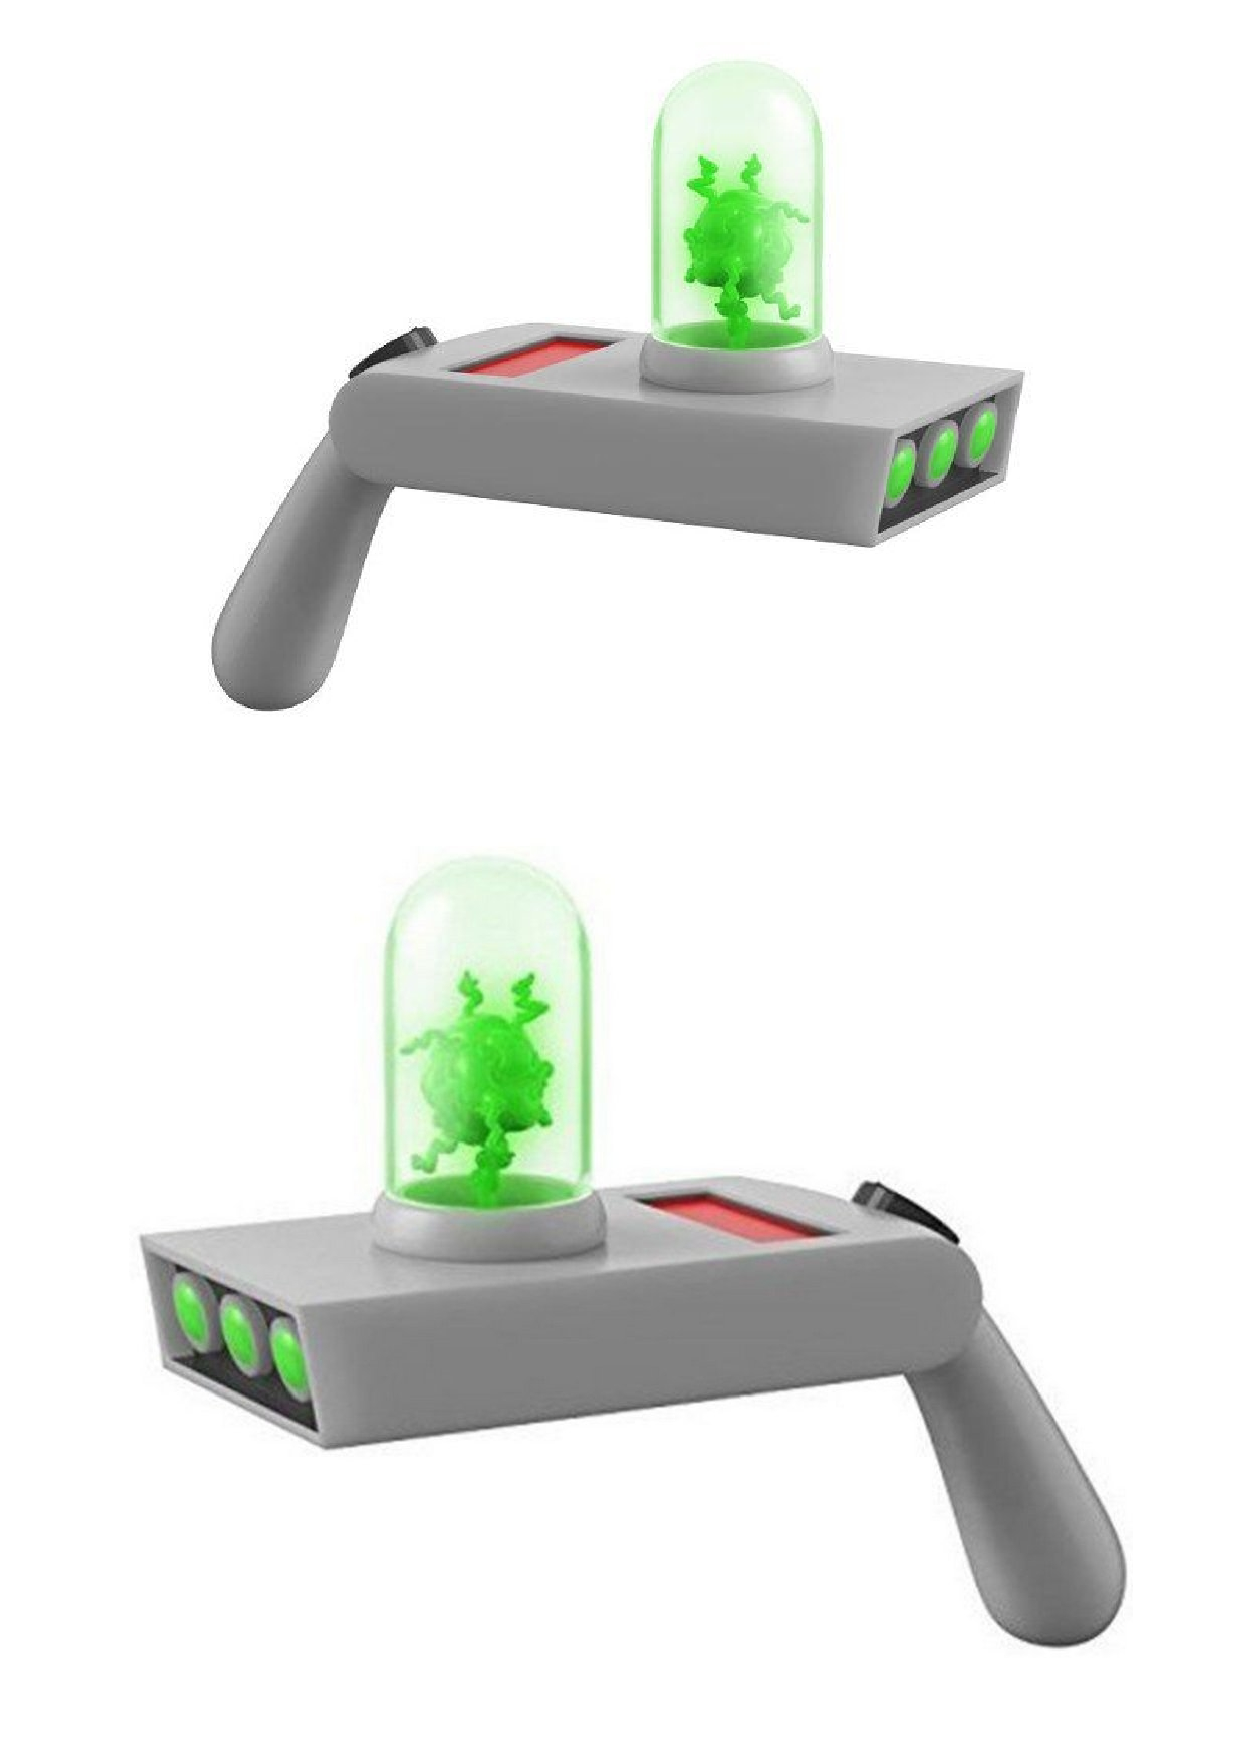
\includepdf[scale=0.8, pages={-}, pagecommand={}]{3-pos-textuais/apendices/ProjeotDaArma.pdf}

% para adicionar o arquivo (que precisar ser PDF) use o comando abaixo, mudando apenas o local do arquivo.

% \includepdf[scale=0.8, pages={-}, pagecommand={}]{Local do arquivo}


\end{apendicesenv}


% ---
% Anexos
% ---
\begin{comment}
\begin{anexosenv}

% Imprime uma página indicando o início dos anexos
\partanexos

% NBR 14724:2011: 3.3: anexo:texto ou documento não elaborado pelo autor, que serve de fundamentação, comprovação e ilustração

% ---
\chapter{Nome anexo 1}
% ---

Um anexo é um documento que não foi elaborado pelo autor, ou seja, o autor apenas anexa. Anexos podem ser tabelas, mapas, diagramas, \textit{datasheets}, manuais e etc. 


% ---
\chapter{Nome anexo 2}
% ---

Um anexo é um documento que não foi elaborado pelo autor, ou seja, o autor apenas anexa. Anexos podem ser tabelas, mapas, diagramas, \textit{datasheets}, manuais e etc. 

% ---
\chapter{Nome anexo 3}
% ---

O autor pode anexar um PDF, traduzido como formato portátil de documento. 

Pode-se fazer uma descrição sucinta do arquivo anexado.
	

\end{anexosenv}
\end{comment}
% ---
% INDICE REMISSIVO
% ---
\phantompart
\printindex


%---------------------------------------------------------------------
%\end{comment}
\end{document}